\titleformat{\chapter}[display]
{\normalfont\huge\bfseries}{Capítulo \thechapter}{0.5em}{\huge}
\titlespacing*{\chapter}{0pt}{-1.25cm}{25pt}
\chapter{Arquitectura e Implementacion}

En este capítulo se describirá la arquitectura de la aplicación, así como las tecnologías utilizadas para su implementación.

\section{Arquitectura}

Se pueden categorizar los tres módulos (\textbf{Adquisición de datos}, \textbf{Procesamiento y análisis}, \textbf{Visualización y Presentación}) de la aplicación mencionados en el capitulo anterior en dos categorias principales:

\begin{itemize}
	\item \textbf{Adquisición de paquetes APRS:} En este módulo se encuentran los componentes encargados de la adquisición de paquetes APRS. Estos componentes se encargan de recibir los paquetes APRS, procesarlos y almacenarlos en la base de datos de la aplicación.

	\item \textbf{Aplicación web APRSINT:} En este módulo se encuentran los componentes encargados del análisis, la interpretación y la visualización, de los datos almacenados en la base de datos de la aplicación. Estos componentes se encargan de presentar la información de manera rápida y cómoda para el usuario.
\end{itemize}

\section{Tecnologías utilizadas (Marco Teórico)}

Como se ha mencionado anteriormente, uno de los objetivos de APRSINT es el de ser una solución accesible y fácil de usar. Para lograr este objetivo, se han seleccionado tecnologías ampliamente utilizadas y bien documentadas. A continuación se describen las tecnologías utilizadas en cada uno de los módulos de la aplicación.
\subsection{Raspberry Pi}

La Raspberry Pi es un \textit{Single board computer (SBC)} u ordenador de placa única desarrollada por la Fundación Raspberry Pi. Las raspberry pi son muy populares en el mundo de la informática y la electrónica por su bajo precio, reducido tamaño y su versatilidad.

\begin{itemize}
	\item \textbf{Bajo precio:} La Raspberry es una opción económica para implementar desde prototipos hasta aplicaciones simples, lo que la hace muy accesible para una amplia gama de usuarios.
	\item \textbf{Bajo Consumo Energético:} Su diseño de bajo consumo energético la hace ideal para aplicaciones que requieren funcionamiento continuo.
	\item \textbf{Versatilidad:} La Raspberry Pi 4 es altamente versátil y puede adaptarse a una variedad de casos de uso, desde servidores ligeros hasta placas de desarrollo para robótica y automatización.
\end{itemize}
Se ha seleccionado la Raspberry Pi 4b\footnote{Cuando se comenzó el proyecto todavía no se habia lanzado la versión 5.} de 8GB de memoria ram como plataforma de hardware para la implementación de la solución, debido a sus características y capacidades.

\subsection{Disco duro ssd}
Los discos duros de estado sólido (SSD) son una alternativa a los discos duros tradicionales (HDD) que ofrecen una mayor velocidad de lectura y escritura, menor consumo energético y mayor durabilidad. Se ha seleccionado un disco duro SSD de 250GB que se haya conectado a la raspberry-pi para almacenar el gran volumen de datos que consume y genera la aplicacion a su velocidad y fiabilidad.

\subsection{Python}
Python es un lenguaje de programación interpretado, de alto nivel y de propósito general. Es ampliamente utilizado en el desarrollo de aplicaciones web, científicas y de análisis de datos debido a su simplicidad, flexibilidad y facilidad de uso. Se ha seleccionado Python como lenguaje de programación principal para la implementación de la solución debido a la gran versatilidad que ofrece y sobretodo por la existencia de extensas librerias de visualización y manejo de grandes volumenes de datos.

\subsection{Dash}
Dash es un framework de Python creado por plotly para la creación de aplicaciones web interactivas y visualizaciones de datos. Dash permite crear aplicaciones web interactivas y visualizaciones de datos atractivas utilizando Python como lenguaje de programación. Dash esta construido encima de React Se ha seleccionado Dash como framework para la implementación de la interfaz web de la aplicación debido a su facilidad de uso y a la gran cantidad de funcionalidades que ofrece. Dash está escrito encima de Plotly.js, React y Flask lo que permite una gran capacidad de customizacion.

\begin{itemize}
	\item \textbf{Interactividad:} Dash permite crear aplicaciones web altamente interactivas, lo que facilita la exploración de datos y la toma de decisiones.
	\item \textbf{Flexibilidad:} Su arquitectura modular y su amplia gama de componentes permiten la creación de aplicaciones web personalizadas y adaptadas a las necesidades específicas del usuario.
	\item \textbf{Integración con Plotly:} Al estar desarrollado por Plotly, Dash ofrece una integración perfecta con las capacidades de visualización de datos de Plotly, lo que permite crear gráficos y visualizaciones muy atractivas.
\end{itemize}

Para crear la aplicación web se consideraron algunas alternativas como Django, Streamlit y PowerBI, sin embargo, Dash fue la opción escogida debido a su extensa capacidad de customizacion y personalizacion de la que carecian las demás opciones.

\subsection{Cosmograph JS}

Cosmograph es una libreria de JavaScript enfocada en la visualización de grandes grafos y redes complejas en aplicaciones web. Permite representar de manera interactiva relaciones entre entidades, facilitando la comprensión y el análisis de datos estructurados.

\begin{itemize}
	\item \textbf{Visualización de Grafos:} Cosmograph ofrece herramientas avanzadas para la representación visual de grafos como lineas temporales, histogramas y búsquedas de nodos, una mayor comprensión y capacidad de análisis de la información.

	\item \textbf{Rendimiento:} Cosmograph a diferencia de otras librerias más populares como Sigma JS transfiere todos los cálculos de posiciones de los nodos y aristas así como la representación gráfica de este a la GPU. Esto permite la visualización de grafos con miles de nodos y aristas sin afectar el rendimiento de la aplicación.

	\item \textbf{Personalización:} Ofrece opciones de personalización para adaptar la apariencia y el comportamiento de los nodos y aristas según las necesidades específicas del usuario.

\end{itemize}

Después de una gran cantidad de pruebas y tras considerar muchas alternativas como Sigma Js, CytoScape y networkx, se acabó eligiendo Cosmograph sobre todo por su rendimiento.

\subsection{PostgreSQL}

PostgreSQL es un sistema de gestión de bases de datos relacional de código abierto y potente, conocido por su fiabilidad, robustez y capacidad para manejar grandes volúmenes de datos. Ofrece una amplia gama de características avanzadas que lo hacen adecuado para aplicaciones web y empresariales exigentes.

\begin{itemize}
	\item \textbf{Fiabilidad y Robustez:} PostgreSQL es conocido por su alta fiabilidad y capacidad para manejar grandes cargas de trabajo sin sacrificar el rendimiento.
	\item \textbf{Escalabilidad:} Es altamente escalable y puede manejar grandes volúmenes de datos y transacciones concurrentes sin problemas.
	\item \textbf{Funcionalidades Avanzadas:} Ofrece una amplia gama de funcionalidades avanzadas, como soporte para transacciones ACID, vistas materializadas, procedimientos almacenados y Full Text Search (búsqueda de indizada).
	\item \textbf{Almacenamiento de datos semiestructurados:} PostgreSQL es capaz de almacenar y manipular datos no estructurados como JSON de manera eficiente, lo que lo hace adecuado para aplicaciones que requieren almacenamiento de datos semiestructurados.
	\item \textbf{Rendimiento:} PostgreSQL ofrece un rendimiento sólido, especialmente en entornos de alta concurrencia y cargas de trabajo intensivas.
\end{itemize}

La elección de PostgreSQL como sistema de gestion de bases de datos se debió a su robustez, facilidad de uso y a la gran cantidad de funcionalidades que ofrece.

\subsection{Sqlalchemy}
SQLAlchemy es una biblioteca de Python que facilita la interacción con bases de datos relacionales utilizando un enfoque orientado a objetos. Permite trabajar con diferentes motores de bases de datos, como PostgreSQL, MySQL, SQLite, entre otros, de una manera consistente y eficiente.

\begin{itemize}
	\item \textbf{Abstracción de la Base de Datos:} SQLAlchemy proporciona una capa de abstracción sobre la base de datos, lo que permite a los desarrolladores interactuar con la base de datos utilizando objetos de python en lugar de consultas SQL directas.
	\item \textbf{Compatibilidad con Múltiples Motores:} Es compatible con una variedad de motores de bases de datos, lo que brinda flexibilidad para trabajar con diferentes sistemas de gestión de bases de datos según las necesidades del proyecto. En este caso se ha utilizado el potor pysycopg2 para la conexión con PostgreSQL.
	\item \textbf{ORM (Mapeo Objeto-Relacional):} Ofrece un ORM potente y flexible que mapea objetos Python a tablas de bases de datos, facilitando el manejo de relaciones entre objetos y la persistencia de datos.
	\item \textbf{Seguridad:} SQLAlchemy proporciona herramientas para prevenir ataques de inyección SQL y otros problemas de seguridad comunes en el manejo de bases de datos.
\end{itemize}

La elección de SQLAlchemy se ha basado en su capacidad para mejorar el proceso de interacción con la base de datos. Permitiendo una estrecha integración entre la base de datos y la aplicación, permitiendo una flexibilidad muy grande a la hora de hacer consultas o inserciones y sobre todo creando una capa de seguridad para evitar ataques.
\subsection{aprslib}
aprslib es una biblioteca de Python que facilita la interacción con el sistema APRS. Permite recibir y decodificar paquetes APRS, así como enviar paquetes APRS a través de la red APRS-IS.
\begin{itemize}
	\item \textbf{Recepción de Paquetes:} aprslib permite recibir paquetes APRS de la red APRS-IS de manera sencilla.
	\item \textbf{Decodificación de Paquetes:} Facilita la decodificación de paquetes APRS, permitiendo extraer información útil como la posición, velocidad y rumbo de los objetos rastreados.
	\item \textbf{Envío de Paquetes:} aprslib permite enviar paquetes APRS a través de la red APRS-IS, lo que facilita la integración con el sistema APRS.
\end{itemize}
Se ha elegido la libreria aprs por su facilidad de uso, su documentación y su capacidad para decodificar los paquetes APRS.
\subsection{AWS}
Amazon Web Services (AWS) es una plataforma de servicios en la nube ofrecida por Amazon. Proporciona servicios de infraestructura informática, almacenamiento, bases de datos, análisis e inteligencia artificial, entre otros.

\begin{itemize}
	\item \textbf{Fiabilidad:} La infraestructura global de AWS está diseñada para ser altamente disponible y resistente a fallos, lo que garantiza la continuidad del servicio y la seguridad de los datos.
	\item \textbf{Variedad de Servicios:} AWS ofrece una amplia gama de servicios, desde almacenamiento y bases de datos hasta aprendizaje automático y análisis de datos, lo que permite a las empresas construir y desplegar una amplia variedad de aplicaciones y soluciones.
	\item \textbf{Flexibilidad:} AWS proporciona opciones flexibles de implementación, incluyendo la capacidad de utilizar infraestructura física, virtual o basada en contenedores, según las necesidades del proyecto.
	\item \textbf{Seguridad:} AWS cuenta con robustas medidas de seguridad para proteger los datos y las aplicaciones, incluyendo controles de acceso, cifrado de datos y protección contra amenazas.
\end{itemize}

La elección de AWS así como los detalles de la implementación en la nube se describirán en la siguiente sección.

\subsection{Supervisord}
Supervisor es un sistema de control de procesos para sistemas operativos tipo Unix, diseñado para iniciar, detener y gestionar procesos de manera sencilla y robusta. Permite supervisar y mantener en funcionamiento aplicaciones y servicios, reiniciándolos automáticamente en caso de fallos o reinicios del sistema.

\begin{itemize}
	\item \textbf{Gestión de Procesos:} Supervisor facilita la gestión de procesos al permitir iniciar, detener, reiniciar y supervisar procesos de manera centralizada.
	\item \textbf{Monitorización:} Supervisor proporciona información detallada sobre el estado de los procesos, incluyendo registros de eventos y estadísticas de rendimiento.
	\item \textbf{Reinicio Automático:} En caso de fallos, Supervisor puede reiniciar automáticamente los procesos afectados, minimizando el tiempo de inactividad y manteniendo la disponibilidad del servicio.
\end{itemize}

Se ha seleccionado Supervidord como gestor de procesos gracias a su facilidad, flexibilidad (permitiendo ejecutar scripts de python directamente) y robustez.
\subsection{Pandas}
Pandas es la libreria de facto de python para el manejo y análisis de datos estructurados. Está escrita sobre numpy (escrito en c) por lo que cuenta con muy buen rendimiento. Esta libreria permite la lectura y escritura de datos en diferentes formatos, la manipulación de datos, la limpieza de datos y la creación de gráficos.
\subsection{Apache Airflow}
Apache Airflow es una plataforma de orquestacion de tareas y flujos de trabajo. Es similar a Cron de Unix pero permite una mayor personalización y control de las tareas que ejecuta. Las tareas se definen en archivos separados facilitando la compartimentalización y ofreciendo una mayor robustez y escalabilidad.
\begin{itemize}
	\item \textbf{Orquestación de Flujos de Trabajo:} Airflow facilita la orquestación de flujos de trabajo complejos al permitir definir tareas y sus dependencias como DAGs, lo que proporciona una visión clara de la lógica de ejecución.
	\item \textbf{Escalabilidad:} Airflow es altamente escalable y puede manejar flujos de trabajo de cualquier tamaño, desde tareas simples hasta flujos de trabajo altamente complejos.
	\item \textbf{Monitoreo y Alertas:} Proporciona una interfaz de usuario web para monitorear el estado de los flujos de trabajo, así como capacidades de alerta para detectar y responder a fallos o retrasos en la ejecución de tareas.
	\item \textbf{Extensibilidad:} Airflow es altamente extensible y permite integrar fácilmente con otros sistemas y herramientas, lo que permite construir flujos de trabajo personalizados que se adapten a las necesidades específicas del proyecto.
\end{itemize}

\section{Adquisición de datos}
En esta sección se describirá con detalle el módulo de adquisición de datos de la aplicación, incluyendo la arquitectura, los componentes y las tecnologías utilizadas.
\subsection{RTL-SDR}
En la primera fase del proyecto se compró un dongle RTL-SDR con el fin de recibir los paquetes APRS y procesarlos a partir de ello. Estos dongles son relativamente baratos oscilando entre los 30 y 100 euros, se conectan mediante usb al ordenador y tienen en la parte superior un conector SMA para conectar una antena. La peculiar de estos dispositivos reside en que son controlables mediante software y se pueden sintonizar en un rango de frecuencias muy amplio (24MHz a 1.7GHz).

Para hacer uso de estos dispositivos se ha de usar software como GQRX, CubicSDR o SDRSharp. Es posible también usar rtl-sdr en la terminal creando posteriormente un microfono virtual para que el software de análisis pueda decodificar los paquetes.

Tras multitud de pruebas fallidas con distintos software de visualización y análisis y software de audio como direwolf, se decidió no continuar por ese camino y probar otras alternativas como la que finalmente se ha implementado el \textbf{APRS-IS} 

\subsection{APRS-IS}
APRS-IS es un sistema que permite la transmisión de mensajes APRS por la red de Internet. La ventaja que ofrece este sistema frente al de recopilar información mediante una antena es que APRS-IS, permite obtener un flujo de datos mucho mayor ya que hay una gran cantidad de antenas y otra ventaja con la que cuenta es que no esta restringido al área que puede recibir la pequeña antena rtl-sdr sino a todo el mundo.

\subsubsection{Infraestructura de la red APRS-IS}
Componentes principales:
\begin{itemize}
	\item \textbf{Trackers o TNC:} Son los emisores de los paquetes APRS, suelen corresponder a estaciones fijas o moviles que envian por radio los paquetes con información de posición, velocidad, rumbo, etc.
	\item \textbf{Digipeaters:} Son estaciones que reciben los paquetes APRS y los retransmiten, permitiendo que los paquetes lleguen a una mayor distancia. Son análogos a los repetidores de internet.
	\item \textbf{I-Gates:} Son estaciones que reciben los paquetes APRS por radio y los envian a la red APRS-IS, permitiendo que los paquetes sean accesibles a través de internet.
	\item \textbf{Servidores APRS-IS:} Son servidores que reciben los paquetes APRS de los I-Gates y los almacenan en una base de datos, permitiendo que los clientes accedan a los paquetes a través de internet. Los servidores APRS-IS suelen estar distribuidos geográficamente para mejorar la disponibilidad y la redundancia.
	\item \textbf{Clientes APRS-IS:} Pueden ser otros servidores, aplicaciones web o aplicaciones móviles que acceden a los servidores APRS-IS para obtener los paquetes APRS y mostrarlos a los usuarios. 
\end{itemize}
Se muestra el flujo de datos de la red APRS-IS en la \Cref{fig:aprs-infra}.
\begin{figure}[h]
	\centering 
	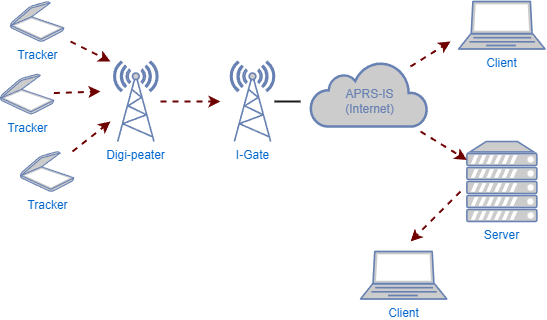
\includegraphics[width=0.85\textwidth]{./Chapter_4/aprs_infra.png}
	\caption{Infrasestructura de la red APRS - APRS-IS.}
	\label{fig:aprs-infra}
\end{figure}

Se ha seleccionado APRS-IS como fuente de datos para la aplicación debido a su facilidad de uso, su disponibilidad y la gran cantidad de información que ofrece.

\begin{figure}[h]
	\centering
	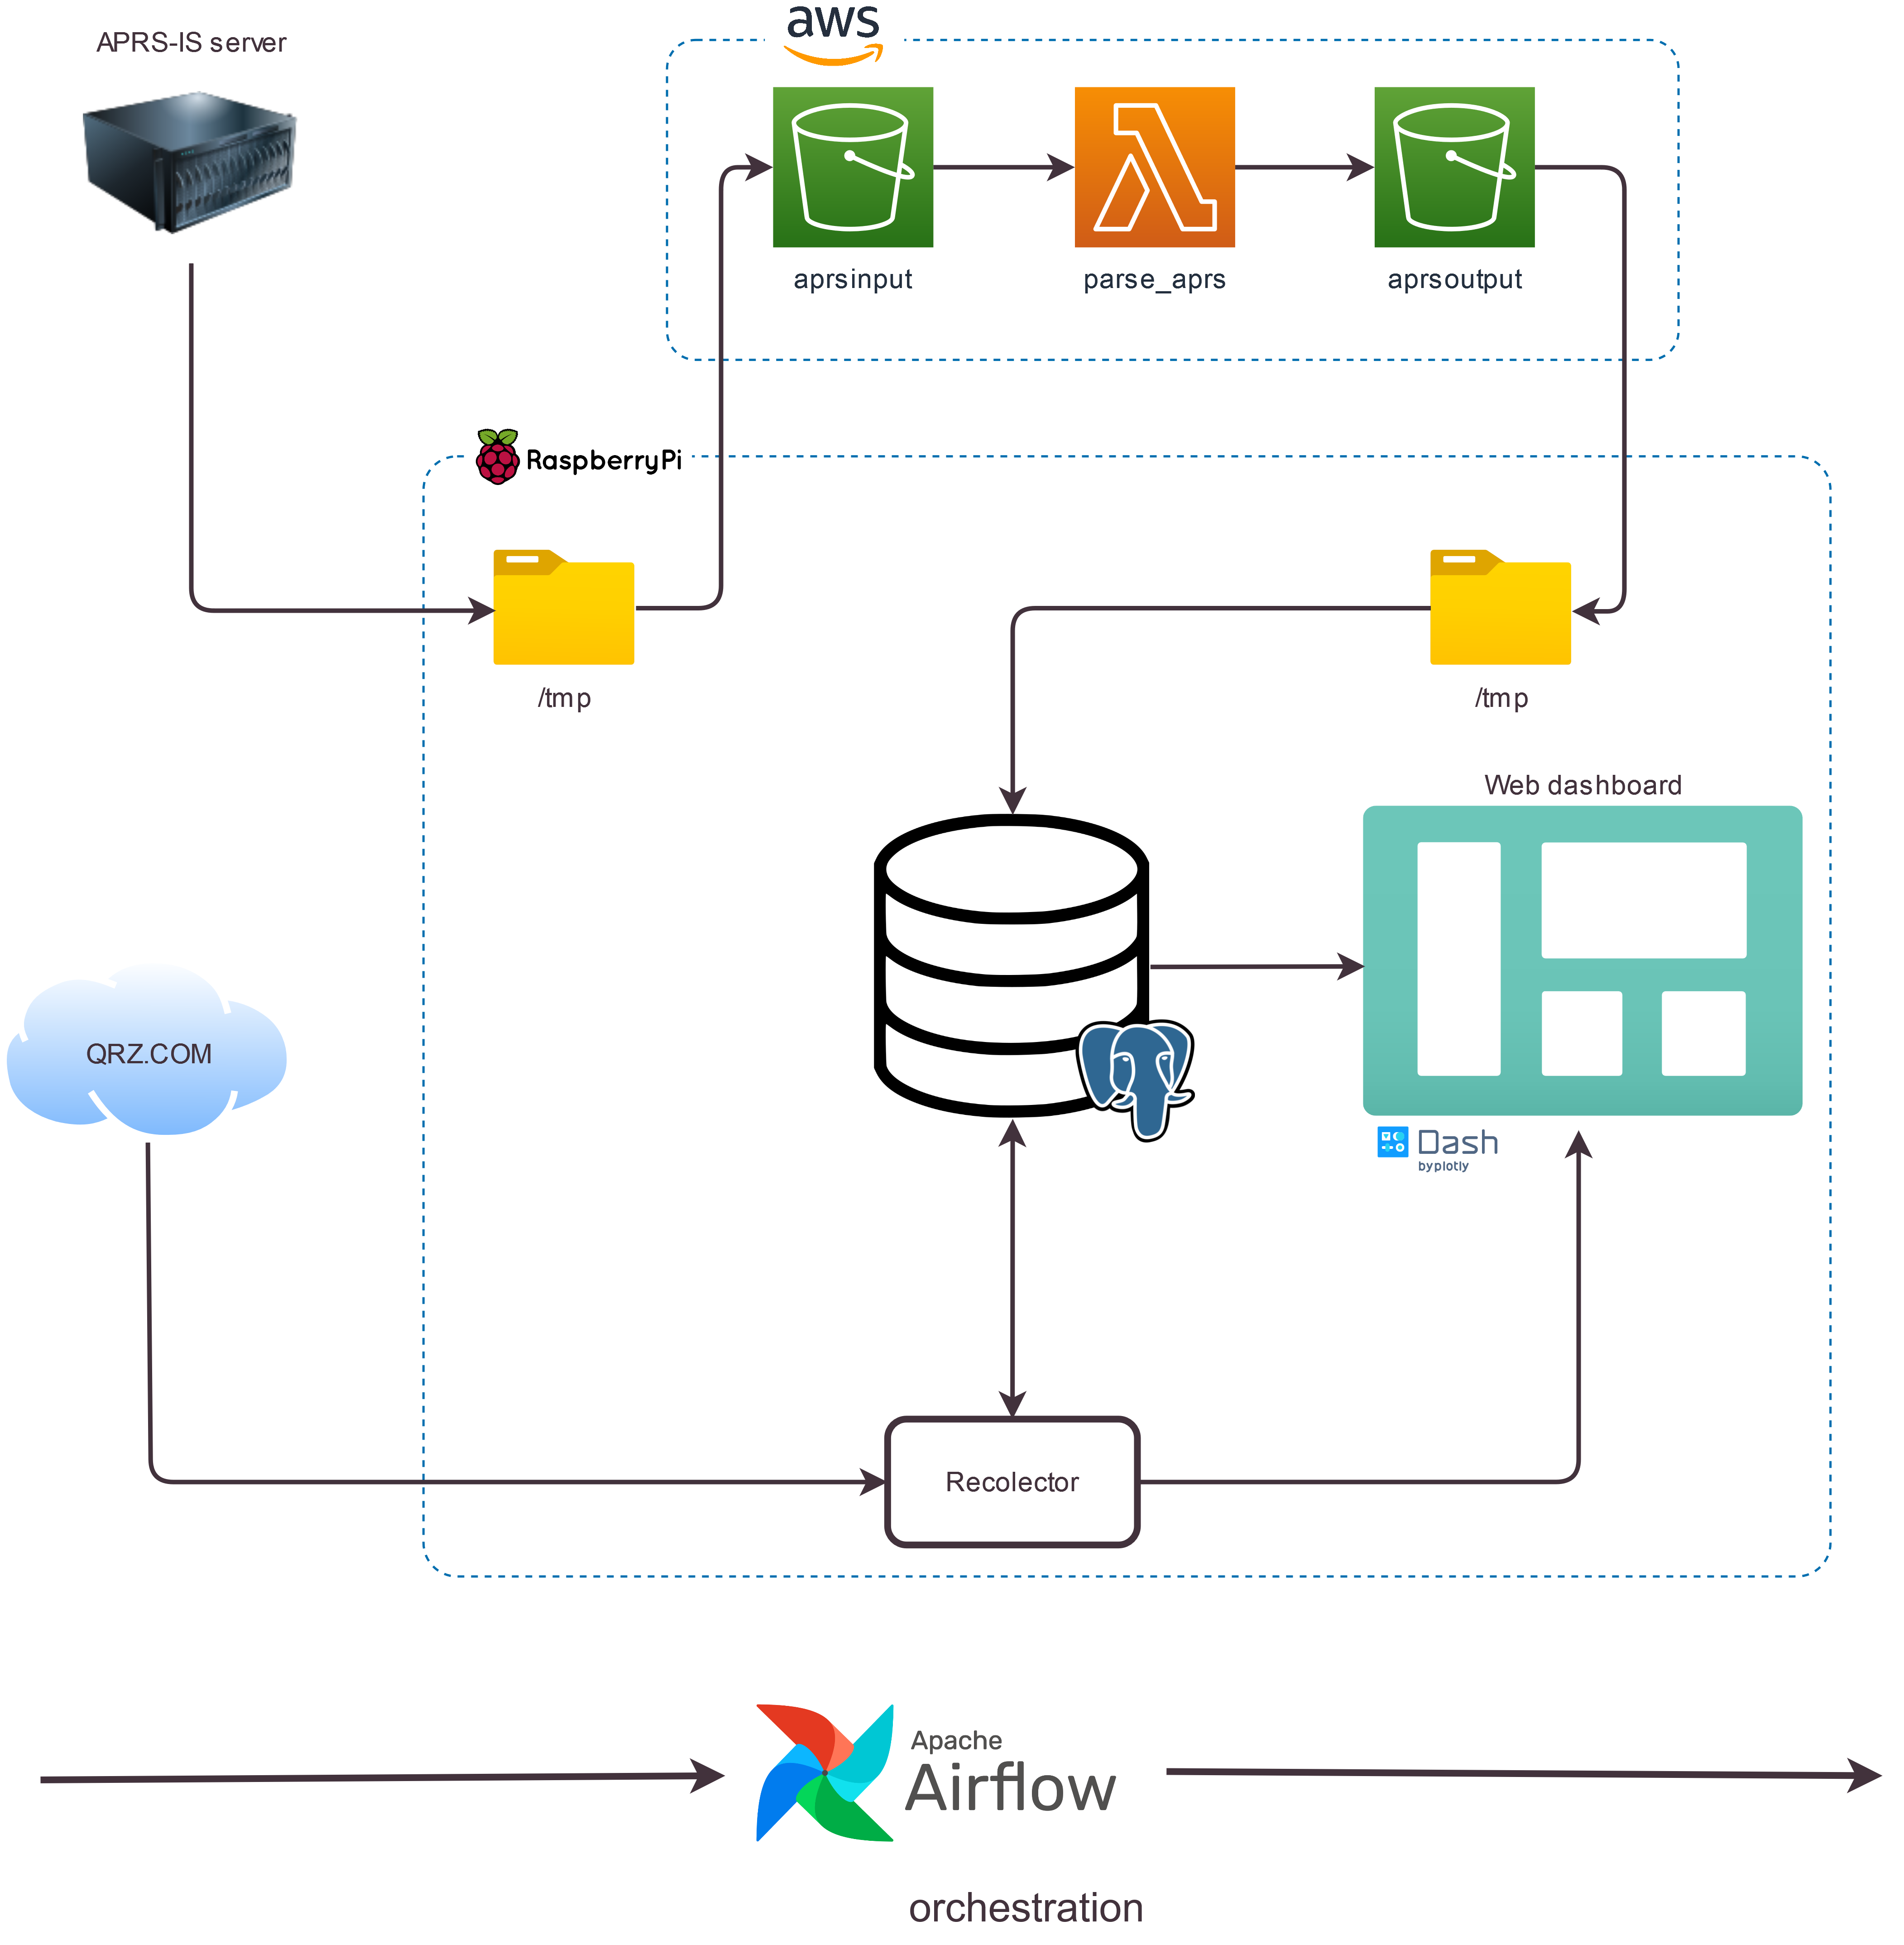
\includegraphics[width=0.85\textwidth]{./Chapter_4/cloud_arch.png}
	\caption{Estructura base de la aplicación.}
	\label{fig:cloud-architecture}
\end{figure}